\documentclass[11pt,a4paper]{article}

\usepackage[T1]{fontenc}
\usepackage[utf8]{inputenc}
\usepackage{amsmath,amsthm,amssymb}
% IBM Plex, as in the Z80 Workbench documents: serif text, sans headings,
% mono code
\usepackage[semibold]{plex-serif}
\usepackage[semibold,scale=0.95]{plex-sans}
\usepackage[scale=0.9]{plex-mono}
\usepackage[italic]{mathastext}
\usepackage{microtype}
\usepackage[margin=1in]{geometry}
\usepackage{array,booktabs,tabularx}
\usepackage[dvipsnames]{xcolor}
\usepackage{tikz}
\usetikzlibrary{positioning,arrows.meta,shapes.geometric,calc,fit,backgrounds}
\usepackage{listings}
\usepackage[most]{tcolorbox}
\usepackage[font=small,labelfont=bf]{caption}
\usepackage{enumitem}
\usepackage{titlesec}
\usepackage[colorlinks,linkcolor=MidnightBlue,citecolor=MidnightBlue,urlcolor=MidnightBlue]{hyperref}
\usepackage[nameinlink]{cleveref}

\titleformat*{\section}{\Large\sffamily\bfseries}
\titleformat*{\subsection}{\large\sffamily\bfseries}
\titleformat*{\paragraph}{\sffamily\bfseries}

% ---------------------------------------------------------------- notation
\newcommand{\ag}[1]{\mathsf{#1}}
\newcommand{\Z}{\ag{Z}}
\newcommand{\Sa}{\ag{S}}
\newcommand{\Add}{\ag{Add}}
\newcommand{\Mul}{\ag{Mul}}
\newcommand{\Dup}{\ag{Dup}}
\newcommand{\Era}{\ag{Era}}
\newcommand{\Lam}{\ag{Lam}}
\newcommand{\App}{\ag{App}}
\newcommand{\Con}{\ag{Con}}
\newcommand{\act}{\mathrel{\bowtie}}
\newcommand{\eqn}{\mathrel{\sim}}
\newcommand{\rul}{\;\Rightarrow\;}
\newcommand{\red}{\;\to\;}
\newcommand{\reds}{\;\to^{*}\;}

% agents = blue, new agents = orange
\definecolor{tfill}{HTML}{DCE9F7}
\definecolor{cfill}{HTML}{FCE8D2}
\definecolor{tline}{HTML}{2F6DB5}
\definecolor{cline}{HTML}{C7701C}
\definecolor{sline}{HTML}{3C8A3A}

\tikzset{
  >=Stealth,
  every picture/.append style={font=\small, baseline=(current bounding box.center)},
  agent/.style={draw=tline, fill=tfill, thick, regular polygon,
    regular polygon sides=3, minimum size=1.3cm, inner sep=0pt,
    font=\small\sffamily},
  newagent/.style={draw=cline, fill=cfill},
  wire/.style={thick},
  lbl/.style={font=\small\itshape, inner sep=2pt},
  pp/.style={circle, fill=black, inner sep=1.4pt},
}
% \Up[style]{name}{position}{text}{arity}: an agent with its principal
% port at the top; auxiliary ports name-1, name-2 from left to right,
% principal port name-0
\newcommand{\Up}[5][]{%
  \node[agent,#1] (#2) at (#3) {#4};
  \coordinate (#2-0) at (#2.corner 1);
  \ifnum#5=1 \coordinate (#2-1) at ($(#2.corner 2)!.5!(#2.corner 3)$);\fi
  \ifnum#5=2 \coordinate (#2-1) at ($(#2.corner 2)!.27!(#2.corner 3)$);
    \coordinate (#2-2) at ($(#2.corner 2)!.73!(#2.corner 3)$);\fi
  \node[pp] at (#2-0) {};}
% \Down: the same with the principal port at the bottom
\newcommand{\Down}[5][]{%
  \node[agent,regular polygon rotate=180,#1] (#2) at (#3) {#4};
  \coordinate (#2-0) at (#2.corner 1);
  \ifnum#5=1 \coordinate (#2-1) at ($(#2.corner 3)!.5!(#2.corner 2)$);\fi
  \ifnum#5=2 \coordinate (#2-1) at ($(#2.corner 3)!.27!(#2.corner 2)$);
    \coordinate (#2-2) at ($(#2.corner 3)!.73!(#2.corner 2)$);\fi
  \node[pp] at (#2-0) {};}
% a free wire end with a name
\newcommand{\fw}[3][above]{\node[lbl,#1] at (#2) {$#3$};}
\newcommand{\ruleto}[1]{\node[font=\Large] at (#1) {$\Rightarrow$};}

\theoremstyle{definition}
\newtheorem{definition}{Definition}
\newtheorem{exercise}{Exercise}
\theoremstyle{plain}
\newtheorem{theorem}{Theorem}
\newtheorem{corollary}{Corollary}

\newtcolorbox{aside}[1]{enhanced, breakable, colback=black!3, colframe=black!35,
  boxrule=0.5pt, arc=2pt, fonttitle=\sffamily\bfseries\small, title={#1},
  coltitle=black, colbacktitle=black!10, left=6pt, right=6pt}

\lstdefinelanguage{inet}{morecomment=[l]{\#}, sensitive=true,
  morekeywords={include}}
\lstset{language=inet, basicstyle=\ttfamily\small, keywordstyle=\bfseries,
  commentstyle=\color{black!55}, columns=fullflexible, keepspaces,
  frame=single, rulecolor=\color{black!30}, xleftmargin=6pt, xrightmargin=6pt,
  aboveskip=8pt, belowskip=8pt, tabsize=8}
\lstdefinestyle{trace}{language={}, basicstyle=\ttfamily\footnotesize}
\lstdefinestyle{plain}{language={}, keywordstyle={}}

\title{\sffamily\bfseries Interaction Nets\\[4pt]
  \large\mdseries A Tutorial Introduction}
\author{}
\date{\today}

\begin{document}
\maketitle

\begin{abstract}
\noindent
An interaction net is a graph in which every node has exactly one
distinguished port, and computation happens only where two such ports meet.
That single restriction, introduced by Yves Lafont in 1990, has striking
consequences. Every rewrite is local and takes constant time; rewrites never
overlap, so they may be done in any order, or all at once, and every order
takes exactly the same number of steps; nothing is ever shared behind the
program's back, so copying and erasing are explicit and there is no need for
a garbage collector. This tutorial develops interaction nets from the
beginning, for readers who know functional programming and the
$\lambda$-calculus. It shows how to write programs as interaction rules, proves
the main property, strong confluence, introduces Lafont's three universal
\emph{interaction combinators}, and then encodes the $\lambda$-calculus,
where interaction nets lead to Lévy's \emph{optimal} reduction and to the
difficult question of when two copying operations should cancel. Every trace
and count in the text comes from a small reducer, \texttt{inet.py}, that runs
the rules exactly as they are written here.
\end{abstract}

\tableofcontents

% =====================================================================
\section{Introduction}

The companion tutorials in this repository describe three machines for the
$\lambda$-calculus. The SECD machine and the Categorical Abstract Machine keep
an \emph{environment} that holds the values of variables, and build
\emph{closures}. Turner's combinator graph reducer removes variables
altogether, and evaluates by rewriting a graph in place. All three have
something in common: they share data through \emph{pointers}. A closure, an
environment or a graph node may be referred to from many places. That is what
makes them efficient, since a shared value is computed once, but it also
means that the machine needs a garbage collector, that a rewrite at one node
may be seen from far away, and that the order of evaluation is fixed by the
machine (the SECD and the CAM evaluate arguments first; the graph reducer
unwinds the spine).

Interaction nets take the opposite position. A net is a graph whose edges are
\emph{wires} between \emph{ports}, and every port is connected to exactly one
wire. A node, called an \emph{agent}, has one distinguished port, its
\emph{principal port}, and a rule applies only where two principal ports meet.
There is no pointer that two parts of a program can hold at the same time: if
a value is needed twice, the net must contain an agent that \emph{copies} it,
and if a value is not needed, an agent that \emph{erases} it.

The idea comes from logic. Girard's linear logic~\cite{girard87} has a
graphical proof system, \emph{proof nets}, in which cut elimination is a local
graph rewrite. Lafont~\cite{lafont90} extracted the computational core of
proof nets and turned it into a programming model. The constraints that come
from logic turn out to be exactly what is needed for good computational
properties:

\begin{enumerate}[itemsep=2pt]
\item \textbf{Locality.} A rewrite touches two agents and the wires attached
  to them, and nothing else. It takes constant time and allocates a bounded
  number of agents.
\item \textbf{Strong confluence.} Two rewrites can never interfere with each
  other. So the order in which they are done does not matter, not only for
  the result but for the \emph{number} of steps.
\item \textbf{Parallelism.} Since rewrites are independent, they can all be
  done at the same time.
\item \textbf{Explicit resources.} Copying and erasing are rules like any
  other. Their cost is visible, and there is no garbage collector.
\end{enumerate}

\noindent
Interaction nets are also the setting in which the $\lambda$-calculus can be
reduced \emph{optimally}, in Lévy's sense~\cite{levy80}: without ever
duplicating a redex. Lamping~\cite{lamping90} found the first such algorithm
in 1990, the same year as Lafont's paper, and it is, in hindsight, an
interaction net.

\paragraph{Plan.} \Cref{sec:nets} defines interaction nets and a textual
notation for them. \Cref{sec:programming} writes programs with them:
arithmetic, pattern matching, copying and erasing. \Cref{sec:properties}
proves strong confluence and looks at what it implies, including what goes
wrong with garbage. \Cref{sec:combinators} presents the three interaction
combinators, which can simulate any interaction net. \Cref{sec:lambda}
encodes the $\lambda$-calculus, meets the problem of sharing under a
$\lambda$, and measures optimal reduction against normal order.
\Cref{sec:implementation} describes how interaction nets are implemented,
and \cref{sec:comparison} compares them with the machines of the companion
tutorials. The tutorial ends with exercises and a reference card.

\paragraph{The reducer.} The directory \texttt{interaction-nets} contains
\texttt{inet.py}, a reducer of about 900 lines of Python. It reads rules and
nets in the notation of \cref{sec:notation}, reduces the net, and prints the
result and the number of interactions, broken down by rule:
\begin{lstlisting}[style=plain]
python3 inet.py add.inet         # run a net
python3 inet.py -t add.inet      # print the net after every interaction
python3 inet.py -r 7 mul.inet    # choose active pairs in random order, seed 7
python3 inet.py -c lam/pred.lam  # a lambda-term, checked against normal order
\end{lstlisting}
\texttt{sh test.sh} checks every count quoted in this text.

% =====================================================================
\section{Interaction nets}\label{sec:nets}

\subsection{Agents, ports and wires}

\begin{definition}
A \emph{signature} $\Sigma$ is a set of symbols, each with an \emph{arity}
$n \ge 0$. An \emph{agent} is an occurrence of a symbol $\alpha$ of arity $n$.
It has $n+1$ \emph{ports}: one \emph{principal port} and $n$ \emph{auxiliary
ports}, numbered $1,\dots,n$.
\end{definition}

\noindent
We draw an agent as a triangle with the principal port at the apex, marked
with a dot, and the auxiliary ports along the base, numbered from left to
right when the apex points up (\cref{fig:agent}).

\begin{definition}
A \emph{net} over $\Sigma$ is a finite set of agents together with a set of
\emph{wires}. A wire connects two ports, and every port is connected to
exactly one wire. A wire may also have one or both ends \emph{free}; the free
ends form the \emph{interface} of the net. A wire may also form a closed loop
with no ports at all.
\end{definition}

\noindent
The interface is how a net talks to the outside world: an input or output
value is attached to it. Note what the definition rules out. A port cannot be
connected to two wires, so an agent cannot be shared, and a wire cannot be
left dangling inside the net, so nothing can be thrown away silently.

\begin{definition}
Two agents whose principal ports are connected by a wire form an
\emph{active pair}, written $\alpha \act \beta$.
\end{definition}

\noindent
An active pair is the interaction-net version of a redex. Since each agent has
only one principal port, an agent belongs to at most one active pair, which
is the key to everything in \cref{sec:properties}.

\begin{figure}[t]
\centering
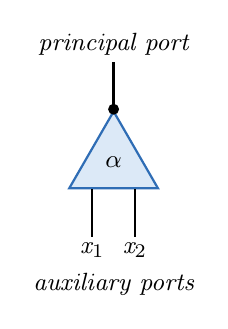
\begin{tikzpicture}
  \Up{a}{0,0}{$\alpha$}{2}
  \draw[wire] (a-0) -- ++(0,.6) node[lbl,above] {principal port};
  \draw[wire] (a-1) -- ++(0,-.6) node[lbl,below] {$x_1$};
  \draw[wire] (a-2) -- ++(0,-.6) node[lbl,below] {$x_2$};
  \node[lbl, align=center] at (0,-1.55) {auxiliary ports};
\end{tikzpicture}
\hspace{2.5cm}
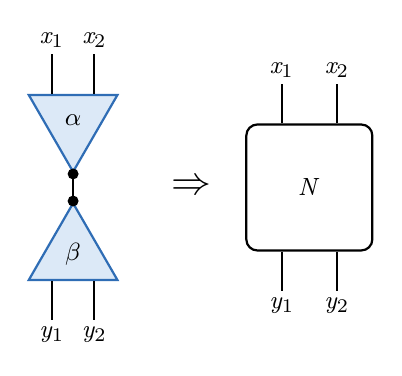
\begin{tikzpicture}
  \Down{a}{0,.85}{$\alpha$}{2}
  \Up{b}{0,-.85}{$\beta$}{2}
  \draw[wire] (a-0) -- (b-0);
  \draw[wire] (a-1) -- ++(0,.5) node[lbl,above] {$x_1$};
  \draw[wire] (a-2) -- ++(0,.5) node[lbl,above] {$x_2$};
  \draw[wire] (b-1) -- ++(0,-.5) node[lbl,below] {$y_1$};
  \draw[wire] (b-2) -- ++(0,-.5) node[lbl,below] {$y_2$};
  \ruleto{1.5,0}
  \node[draw, thick, rounded corners, minimum width=1.6cm,
        minimum height=1.6cm] (n) at (3,0) {$N$};
  \draw[wire] ([xshift=-.35cm]n.north) -- ++(0,.5) node[lbl,above] {$x_1$};
  \draw[wire] ([xshift=.35cm]n.north) -- ++(0,.5) node[lbl,above] {$x_2$};
  \draw[wire] ([xshift=-.35cm]n.south) -- ++(0,-.5) node[lbl,below] {$y_1$};
  \draw[wire] ([xshift=.35cm]n.south) -- ++(0,-.5) node[lbl,below] {$y_2$};
\end{tikzpicture}
\caption{Left: an agent of arity 2. Right: an interaction rule replaces an
active pair $\alpha\act\beta$ by a net $N$ with the same interface.}
\label{fig:agent}
\end{figure}

\subsection{Interaction rules}

\begin{definition}
An \emph{interaction rule} $\alpha \act \beta \rul N$ replaces an active pair
of agents $\alpha$ and $\beta$ by a net $N$ whose interface consists of the
wires $x_1,\dots,x_n$ and $y_1,\dots,y_m$ that were attached to the auxiliary
ports of $\alpha$ and $\beta$ (\cref{fig:agent}). An \emph{interaction
system} is a signature with a set of rules, such that there is \emph{at most
one} rule for each unordered pair of symbols. A rule for $\alpha\act\beta$ is
also a rule for $\beta\act\alpha$, read the other way round, and a rule for
$\alpha \act \alpha$ must be symmetric.
\end{definition}

\noindent
Three features of this definition matter.

\begin{description}[itemsep=2pt, font=\normalfont\itshape]
\item[Linearity.] The interface is preserved exactly: each wire that was
  attached to $\alpha$ or $\beta$ is attached to exactly one port of $N$ (or
  to another such wire). A rule can neither copy a wire nor drop one.
\item[Binary interaction.] A rule looks at two agents and no more. It cannot
  ask what is attached to their auxiliary ports.
\item[No ambiguity.] Each active pair has at most one rule that applies to it.
\end{description}

\noindent
Lafont's original definition also asks that $N$ contain no active pair. This
is a convenience rather than a necessity, and we will break it once, on
purpose, in \cref{sec:garbage}.

A net with no active pairs is in \emph{normal form}. A net may also contain an
active pair for which there is no rule; then the computation is stuck, which
plays the role of a run-time type error.

\subsection{A textual notation}\label{sec:notation}

Pictures are good for intuition but bad for calculation. We use the term
notation of Lafont, as developed by Fernández and Mackie~\cite{fm99}.

\paragraph{Terms.} A net in which every agent's principal port points
``upwards'' towards the root is a tree, and can be written as a term:
$\alpha(t_1,\dots,t_n)$ is an agent $\alpha$ whose auxiliary ports are
connected to the principal ports of $t_1,\dots,t_n$ (or to wires, if $t_i$ is
a name). So $\Sa(\Sa(\Z))$ is a chain of three agents, with the principal
port of the outermost $\Sa$ free.

\paragraph{Wires.} A lower-case name stands for a wire. A name that occurs
twice is a wire between the two places, and a name that occurs once is a free
wire, part of the interface. In $\Add(r, y)$, the agent's two auxiliary ports
are attached to the wires $r$ and $y$.

\paragraph{Equations.} A net that is not a tree is a set of trees whose
principal ports (the roots) are connected to each other or to wires. We write
$t \eqn u$ to connect the root of $t$ to the root of $u$. An equation between
two agents is an active pair; an equation $x \eqn t$ attaches the root of $t$
to the wire $x$.

\paragraph{Rules.} A rule is written
\[
  \alpha(x_1,\dots,x_n) \act \beta(y_1,\dots,y_m) \rul e_1,\ \dots,\ e_k
\]
where the $x_i$ and $y_j$ are distinct names and $e_1,\dots,e_k$ are
equations. Linearity becomes a syntactic condition: each $x_i$ and $y_j$
occurs exactly once on the right, and every other name occurs there exactly
twice.

\medskip\noindent
For example, here is a net for $2+2$, which we will meet again in a moment:
\[
  \Add(r, \Sa(\Sa(\Z))) \eqn \Sa(\Sa(\Z))
\]
It has one active pair, between $\Add$ and the outer $\Sa$ on the right, and
one free wire, $r$, where the result will appear. In the files read by
\texttt{inet.py} the symbol $\act$ is written \texttt{><}, $\rul$ is written
\texttt{=>}, and $\eqn$ is written \texttt{\char`\~}. A line that is not a
rule is part of the net, and \texttt{include} reads another file.

\subsection{Reduction}

Reduction is just repeated application of rules:
\[
  N \red N' \quad\text{if $N'$ is $N$ with one active pair replaced by the
  right-hand side of its rule.}
\]
Nothing else changes: no other agent is looked at, nothing is copied, and the
interface of $N$ is the interface of $N'$. In the term notation, applying a
rule $\alpha(\vec x) \act \beta(\vec y) \rul \Delta$ to an equation
$\alpha(\vec t) \eqn \beta(\vec u)$ replaces it by the equations $\Delta$
with $\vec t$ for $\vec x$ and $\vec u$ for $\vec y$. An equation $x \eqn t$
in which $x$ also occurs elsewhere is then resolved by putting $t$ in the
other occurrence of $x$.

% =====================================================================
\section{Programming with interaction nets}\label{sec:programming}

\subsection{Constructors and functions}

Take the natural numbers in unary: $\Z$ of arity 0 and $\Sa$ of arity 1. As
data, their principal ports face their \emph{user}: $\Sa(x)$ offers itself to
whoever is connected above it and holds the predecessor $x$ below.

A function becomes an agent whose principal port faces the argument it
inspects. Addition
\[
  \mathit{add}\ \Z\ y = y, \qquad
  \mathit{add}\ (\Sa\ x)\ y = \Sa\ (\mathit{add}\ x\ y)
\]
inspects its first argument, so $\Add$ has its principal port there, and two
auxiliary ports, one for the result $r$ and one for the second argument $y$.
There is one rule for each constructor (\cref{fig:add}):
\begin{lstlisting}
Add(r, y) >< Z     => r ~ y
Add(r, y) >< S(x)  => r ~ S(w), x ~ Add(w, y)
\end{lstlisting}
The first rule connects the result straight to $y$; both agents disappear.
The second moves the $\Sa$ to the result and the $\Add$ one step down,
connected to $x$ by its principal port. If $x$ is a number, a new active pair
has appeared.

\begin{figure}[t]
\centering
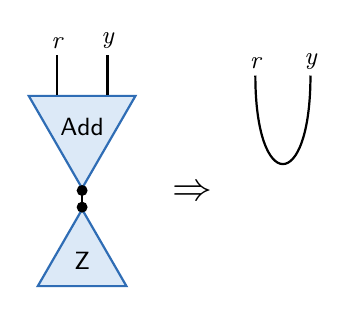
\begin{tikzpicture}
  \Down{a}{0,.85}{Add}{2}
  \Up{s}{0,-.85}{$\Z$}{0}
  \draw[wire] (a-0) -- (s-0);
  \draw[wire] (a-1) -- ++(0,.5) node[lbl,above] {r};
  \draw[wire] (a-2) -- ++(0,.5) node[lbl,above] {y};
  \ruleto{1.4,0}
  \draw[wire] (2.2,1.5) node[lbl,above] {r} .. controls (2.2,0) and (2.9,0)
     .. (2.9,1.5) node[lbl,above] {y};
\end{tikzpicture}
\hspace{1.6cm}
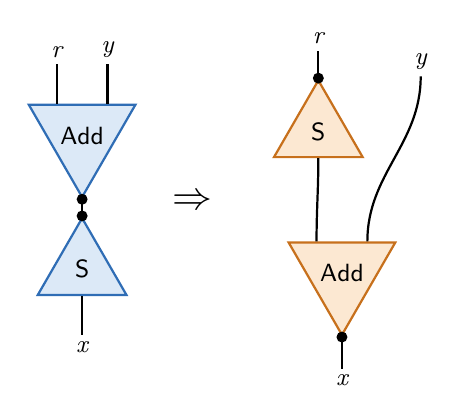
\begin{tikzpicture}
  \Down{a}{0,.85}{Add}{2}
  \Up{s}{0,-.85}{$\Sa$}{1}
  \draw[wire] (a-0) -- (s-0);
  \draw[wire] (a-1) -- ++(0,.5) node[lbl,above] {r};
  \draw[wire] (a-2) -- ++(0,.5) node[lbl,above] {y};
  \draw[wire] (s-1) -- ++(0,-.5) node[lbl,below] {x};
  \ruleto{1.4,0}
  \Up[newagent]{s2}{3,.9}{$\Sa$}{1}
  \Down[newagent]{a2}{3.3,-.9}{Add}{2}
  \draw[wire] (s2-0) -- ++(0,.35) node[lbl,above] {r};
  \draw[wire] (s2-1) to[out=-90,in=90] (a2-1);
  \draw[wire] (a2-2) to[out=90,in=-90] (4.3,1.6) node[lbl,above] {y};
  \draw[wire] (a2-0) -- ++(0,-.4) node[lbl,below] {x};
\end{tikzpicture}
\caption{The two rules for addition. Interaction moves the $\Add$ agent down
the first argument, leaving a copy of each $\Sa$ on the result wire.}
\label{fig:add}
\end{figure}

Here is $2+2$, as traced by \texttt{inet.py -t add.inet}. Each line is the
net after one more interaction; the reducer names internal wires
\texttt{w1}, \texttt{w2},~\dots
\begin{lstlisting}[style=trace]
   0  S(S(Z)) ~ Add(r, S(S(Z)))
   1  r ~ S(w1),  S(Z) ~ Add(w1, S(S(Z)))
   2  r ~ S(S(w1)),  Z ~ Add(w1, S(S(Z)))
   3  r ~ S(S(S(S(Z))))
interactions: 3 (Add-S 2, Add-Z 1)
\end{lstlisting}
Notice line 1. The result wire already carries an $\Sa$, before the addition
has finished: the output is produced incrementally, as in a lazy language.
In general $m+n$ takes $m+1$ interactions.

\subsection{Pattern matching on two arguments}

Since a rule sees only two agents, a function can inspect only \emph{one}
argument at a time: the one at its principal port. A function that matches on
two arguments must do it in two steps, with an intermediate agent that
remembers what it found in the first. For
\[
  \mathit{max}\ \Z\ y = y, \qquad
  \mathit{max}\ (\Sa\,x)\ \Z = \Sa\,x, \qquad
  \mathit{max}\ (\Sa\,x)\ (\Sa\,y) = \Sa\,(\mathit{max}\ x\ y)
\]
the agent $\ag{Max}$ inspects the first argument; when it finds an $\Sa$ it
turns into $\ag{Max1}$, which holds the predecessor and turns its principal
port towards the second argument:
\begin{lstlisting}
Max(r, y) >< Z      => r ~ y
Max(r, y) >< S(x)   => y ~ Max1(r, x)
Max1(r, x) >< Z     => r ~ S(x)
Max1(r, x) >< S(y)  => r ~ S(w), x ~ Max(w, y)
\end{lstlisting}
This is exactly the compilation of pattern matching into a decision tree, or
the curried view of a two-argument function, with one agent per state.

\subsection{Copying and erasing}

Multiplication shows the two things that make interaction nets different from
term rewriting:
\[
  \mathit{mul}\ \Z\ y = \Z, \qquad
  \mathit{mul}\ (\Sa\,x)\ y = \mathit{add}\ (\mathit{mul}\ x\ y)\ y
\]
The first equation \emph{drops} $y$, and the second uses it \emph{twice}. A
rule cannot do either, because it must connect each wire exactly once. So we
need two more agents: $\Era$, of arity 0, which erases what it meets, and
$\Dup$, of arity 2, which copies what it meets onto its two auxiliary ports.
They are defined, like everything else, by rules for each constructor:
\begin{lstlisting}
Mul(r, y) >< Z     => r ~ Z, y ~ Era
Mul(r, y) >< S(x)  => y ~ Dup(a, b), x ~ Mul(m, a), m ~ Add(r, b)

Dup(a, b) >< Z     => a ~ Z, b ~ Z
Dup(a, b) >< S(x)  => a ~ S(a1), b ~ S(b1), x ~ Dup(a1, b1)
Era >< Z           =>
Era >< S(x)        => x ~ Era
\end{lstlisting}
In the second $\Mul$ rule the equation $y \eqn \Dup(a,b)$ turns the principal
port of a new $\Dup$ towards $y$, so that it copies $y$ one constructor at a
time, sending one copy to the recursive $\Mul$ and the other to the $\Add$.
Copying is \emph{incremental}: a $\Dup$ passes through an $\Sa$ by making two
$\Sa$ and moving on, so a copy of a number can be used before it is complete,
and if one copy is never used, an $\Era$ will meet it and stop it. The
complete trace of $2\times 3$ takes 20 interactions; here are its first
lines:
\begin{lstlisting}[style=trace]
   0  S(S(Z)) ~ Mul(r, S(S(S(Z))))
   1  S(Z) ~ Mul(Add(r, w1), w2),  Dup(w2, w1) ~ S(S(S(Z)))
   2  Z ~ Mul(Add(Add(r, w1), w2), w3),  Dup(Dup(w3, w2), w1) ~ S(S(S(Z)))
   3  Add(Add(r, w1), w2) ~ Z,  Dup(Dup(Era, w2), w1) ~ S(S(S(Z)))
   ...
  20  r ~ S(S(S(S(S(S(Z))))))
interactions: 20 (Add-S 3, Add-Z 2, Dup-S 6, Dup-Z 2, Era-S 3, Era-Z 1,
                  Mul-S 2, Mul-Z 1)
\end{lstlisting}
After step 2 the second argument is about to be copied by a tree of two
$\Dup$ agents, one of whose outputs will be erased. Counting each kind of
interaction for $m \times n$ gives the cost
\[
  \underbrace{(m+1)}_{\Mul} + \underbrace{m(n+1)}_{\Dup}
  + \underbrace{\tfrac12 nm(m-1) + m}_{\Add} + \underbrace{(n+1)}_{\Era},
\]
which is 20 for $2\times 3$ and 25 for $3\times 2$. Copying and erasing are
part of the cost of the program, and are counted like any other step.

\begin{aside}{Data structures with holes}
A wire has two ends, and nothing says that both must be inside the same
data structure. A list with a free wire in place of its final $\ag{Nil}$ is a
\emph{difference list}: the free end gives constant-time access to the end
of the list, and appending is a single connection. Functional languages need
a special representation to get this; in an interaction net it is simply a
net with two interface wires. \Cref{ex:dlist} asks you to write the rules.
\end{aside}

% =====================================================================
\section{Properties}\label{sec:properties}

\subsection{Strong confluence}

\begin{theorem}[Lafont~\cite{lafont90}]\label{thm:confluence}
Interaction-net reduction has the \emph{one-step diamond property}: if
$N \red N_1$ and $N \red N_2$ with $N_1 \ne N_2$, then there is a net $M$
with $N_1 \red M$ and $N_2 \red M$.
\end{theorem}

\begin{proof}
The two steps rewrite two active pairs, $P_1$ and $P_2$. They are different
pairs, since a pair has only one rule and so one result. And they are
\emph{disjoint}: an agent belongs to at most one active pair, because it has
only one principal port. A rule only replaces its own pair and reconnects the
wires that were attached to the pair's auxiliary ports. So in $N_1$ the pair
$P_2$ is still present, unchanged (some of the wires around it may now lead
to different places, but the rule for $P_2$ does not look at them), and the
same holds for $P_1$ in $N_2$. Rewriting $P_2$ in $N_1$ and $P_1$ in $N_2$
gives the same net $M$, since both replace $P_1$ and $P_2$ by their
right-hand sides and make the same connections.
\end{proof}

\noindent
The proof is three lines long, and yet it is the most important fact about
interaction nets. In the $\lambda$-calculus the corresponding diamond fails,
because a $\beta$-step can copy or erase another redex. That is why the
Church--Rosser theorem is hard there and why the choice of evaluation order
matters so much. In an interaction net, no rule can copy or erase an active
pair, because a rule never looks past the two agents it rewrites. A standard
argument on one-step diamonds then gives:

\begin{corollary}\label{cor:length}
If a net $N$ has a normal form, it is unique, every reduction sequence from
$N$ reaches it, and every such sequence has the same length.
\end{corollary}

\noindent
So in an interaction net there are no good and bad evaluation orders. The
number of steps is a property of the net, not of the strategy. You can see
this with \texttt{inet.py -r}, which picks active pairs in random order:
\begin{lstlisting}[style=trace]
$ for s in 1 2 3; do python3 inet.py -q -r $s mul.inet; done
interactions: 20 (Add-S 3, Add-Z 2, Dup-S 6, Dup-Z 2, Era-S 3, Era-Z 1, Mul-S 2, Mul-Z 1)
interactions: 20 (Add-S 3, Add-Z 2, Dup-S 6, Dup-Z 2, Era-S 3, Era-Z 1, Mul-S 2, Mul-Z 1)
interactions: 20 (Add-S 3, Add-Z 2, Dup-S 6, Dup-Z 2, Era-S 3, Era-Z 1, Mul-S 2, Mul-Z 1)
\end{lstlisting}
Not just the total but the count for each rule is the same in every order.
Only the peak memory use, the number of agents alive at once, depends on the
order.

\subsection{Parallelism}

Because active pairs are disjoint, any set of them can be rewritten at the
same time. A parallel implementation needs no locks on agents, only care
where two rewrites reconnect the two ends of the same wire. And by
\cref{cor:length}, a parallel reducer does exactly the same total work as a
sequential one. HVM~\cite{hvm} uses this to run interaction nets on GPUs, with
thousands of active pairs rewritten at once.

\subsection{Deadlock}

A net can be in normal form without being a value. The simplest case is a
\emph{vicious circle}: a cycle of agents, each with its principal port
connected to an auxiliary port of the next, so that no two principal ports
can ever meet. The net $x \eqn \Sa(x)$ is one: a single $\Sa$ whose principal
port is wired to its own auxiliary port. No rule applies, and none ever will.
Lafont gives a type discipline that rules out vicious circles for nets built
in a structured way; for the $\lambda$-calculus encoding of
\cref{sec:lambda}, they appear when the encoding is used incorrectly, and we
will see one.

\subsection{Garbage and divergence}\label{sec:garbage}

\Cref{cor:length} has a price. Since every reduction to normal form has the
same length, the reducer cannot save work by \emph{not} reducing garbage, as
a lazy language does. Consider $0 \times \infty$, where $\infty$ is produced
by an agent that generates $\Sa$'s for ever (this rule deliberately creates
an active pair on its right-hand side):
\begin{lstlisting}
Inf(r) >< Go => r ~ S(w), Inf(w) ~ Go
Mul(r, y) ~ Z,  Inf(y) ~ Go
\end{lstlisting}
In random order the $\Mul\act\Z$ pair is soon chosen (with seed 1, at the
first step), the answer $r \eqn \Z$ appears, and the $\Era$ produced by that
rule eats the $\Sa$'s as fast as they are produced. But the reduction never ends:
\begin{lstlisting}[style=trace]
$ python3 inet.py -q -r 1 -n 1000 inf.inet
stopped after 1000 interactions
interactions: 1000 (Era-S 499, Inf-Go 500, Mul-Z 1)
\end{lstlisting}
With the reducer's default order, a stack of active pairs, it is worse still:
the $\ag{Inf}$ pair is always the most recent, and the $\Mul$ pair is never
chosen at all. A net with an infinite reduction has no normal form, by
\cref{cor:length}, and an unfair strategy may never even produce the part of
the answer that exists.

The remedy is the same as in the $\lambda$-calculus: do not ask for the normal
form. A \emph{weak} or \emph{lazy} strategy~\cite{fm99} rewrites only the active
pairs that the interface depends on. Starting from an interface wire, it
follows principal ports until it finds an active pair, rewrites it, and
starts again; it stops when the agent at the interface is a constructor (for
weak head normal form) or when the whole tree below the interface is in
normal form. Garbage that the interface does not reach is never reduced. We
will measure what this saves for the $\lambda$-calculus in
\cref{sec:measure}.

% =====================================================================
\section{Interaction combinators}\label{sec:combinators}

Every example so far has needed its own agents and its own copying and
erasing rules. Lafont asked whether a \emph{fixed} small set of agents could
simulate all of them, as $\ag{S}$ and $\ag{K}$ simulate the
$\lambda$-calculus. The answer~\cite{lafont97} is three agents and six rules:
a \emph{constructor} $\gamma$ and a \emph{duplicator} $\delta$, both of arity
2, and an \emph{eraser} $\varepsilon$ of arity 0. Their rules follow one
pattern: two agents with the same symbol \emph{annihilate}, and two with
different symbols \emph{commute}, each passing through the other.
\begin{lstlisting}
Con(a, b) >< Con(c, d)  => a ~ d, b ~ c
Dup(a, b) >< Dup(c, d)  => a ~ c, b ~ d
Era >< Era              =>
Con(a, b) >< Dup(c, d)  => a ~ Dup(p, q), b ~ Dup(r, s),
                           c ~ Con(p, r), d ~ Con(q, s)
Era >< Con(a, b)        => a ~ Era, b ~ Era
Era >< Dup(a, b)        => a ~ Era, b ~ Era
\end{lstlisting}
Here \texttt{Con} is $\gamma$, \texttt{Dup} is $\delta$ and \texttt{Era} is
$\varepsilon$. The difference between the two annihilations is essential:
$\gamma$ crosses its wires and $\delta$ does not (in Lafont's notation,
$\gamma[x,y] \act \gamma[y,x]$ but $\delta[x,y]\act\delta[x,y]$). The
commutation $\gamma \act \delta$ is the general pattern for copying: the
$\delta$ goes through the $\gamma$ and comes out as two $\delta$'s, one on
each auxiliary port of the $\gamma$, and the $\gamma$ comes out as two
$\gamma$'s, one for each copy (\cref{fig:comm}).

\begin{figure}[t]
\centering
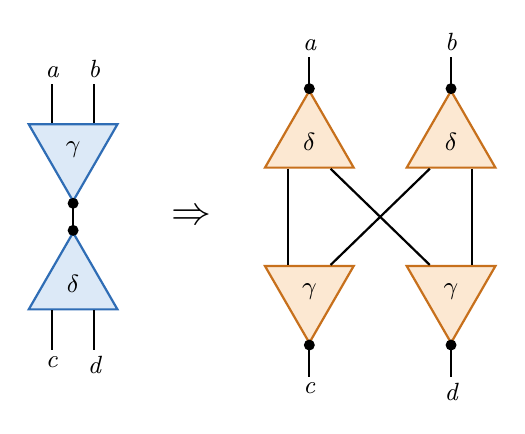
\begin{tikzpicture}
  \Down{a}{0,.85}{$\gamma$}{2}
  \Up{b}{0,-.85}{$\delta$}{2}
  \draw[wire] (a-0) -- (b-0);
  \draw[wire] (a-1) -- ++(0,.5) node[lbl,above] {a};
  \draw[wire] (a-2) -- ++(0,.5) node[lbl,above] {b};
  \draw[wire] (b-1) -- ++(0,-.5) node[lbl,below] {c};
  \draw[wire] (b-2) -- ++(0,-.5) node[lbl,below] {d};
  \ruleto{1.5,0}
  \Up[newagent]{d1}{3,.95}{$\delta$}{2}
  \Up[newagent]{d2}{4.8,.95}{$\delta$}{2}
  \Down[newagent]{g1}{3,-.95}{$\gamma$}{2}
  \Down[newagent]{g2}{4.8,-.95}{$\gamma$}{2}
  \draw[wire] (d1-0) -- ++(0,.4) node[lbl,above] {a};
  \draw[wire] (d2-0) -- ++(0,.4) node[lbl,above] {b};
  \draw[wire] (g1-0) -- ++(0,-.4) node[lbl,below] {c};
  \draw[wire] (g2-0) -- ++(0,-.4) node[lbl,below] {d};
  \draw[wire] (d1-1) -- (g1-1);
  \draw[wire] (d1-2) -- (g2-1);
  \draw[wire] (d2-1) -- (g1-2);
  \draw[wire] (d2-2) -- (g2-2);
\end{tikzpicture}
\caption{Commutation $\gamma\act\delta$: each agent passes through the other
and is copied. The two copies of $\gamma$ are joined to the two copies of
$\delta$ in a square.}
\label{fig:comm}
\end{figure}

\begin{theorem}[Lafont~\cite{lafont97}]
Every interaction system can be translated into the interaction combinators:
each agent becomes a fixed net of $\gamma$, $\delta$ and $\varepsilon$, and
each interaction becomes a bounded number of combinator interactions.
\end{theorem}

\noindent
The proof is constructive but intricate; we only sketch the idea. With
$\gamma$ one builds binary trees that pack several wires into one
(\emph{multiplexers}) and unpack them again. An agent's symbol is encoded by a
pattern of wires, so that when two encoded agents meet, their trees
annihilate and connect their contents in a way that depends on both symbols.
The right-hand sides of the rules, which may be arbitrary nets, are kept in
the encoding of the agents and copied with $\delta$ as needed. The role of
the interaction combinators is thus the same as the role of $\ag{S}$ and
$\ag{K}$: a minimal universal instruction set, of theoretical importance, and
increasingly a practical target (HVM's runtime is built on a close variant
of them).

They also give a first glimpse of the $\lambda$-calculus. Write an abstraction
as $\gamma(x, b)$ (variable, body) and an application as $\gamma(r, a)$
(result, argument), with the application's principal port facing the
function. Then $\gamma(x,b) \act \gamma(r,a)$ annihilates into $x \eqn a$ and
$b \eqn r$: the argument is connected to the variable and the body to the
result. That is $\beta$-reduction, in one interaction. A variable used twice
is copied with a $\delta$. Here is $(\lambda x.\,x\,x)\,(\lambda y.\,y)$:
\begin{lstlisting}[style=trace]
$ python3 inet.py -t selfapp.inet
   0  Con(Dup(Con(w1, w2), w2), w1) ~ Con(out, Con(w3, w3))
   1  Dup(Con(out, w1), w1) ~ Con(w2, w2)
   2  Con(out, Con(w1, w2)) ~ Con(w3, w4),  Dup(w4, w2) ~ Dup(w3, w1)
   3  Dup(out, w1) ~ Dup(Con(w2, w1), w2)
   4  out ~ Con(w1, w1)
\end{lstlisting}
The result $\Con(w_1,w_1)$ is $\lambda w.\,w$. Step 1 is $\beta$; step 2
copies the identity; step 3 is the second $\beta$; and in step 4 two
$\delta$'s annihilate. That last step is where a single $\delta$ is not
enough in general, as the next section explains.

% =====================================================================
\section{The \texorpdfstring{$\lambda$}{lambda}-calculus}\label{sec:lambda}

From now on we use named agents rather than the combinators, so that nets
are easier to read. Their rules are in \texttt{lambda.inet}, and
\texttt{inet.py} translates a $\lambda$-term in a \texttt{.lam} file into a
net over them. The syntax is that of the \texttt{graph/} tutorial: $\lambda$
is \verb|\|, and a file may begin with definitions \texttt{f x y = M;}, which
are expanded at each use.

\subsection{Linear terms}

A term is \emph{linear} if every bound variable occurs exactly once. Linear
terms need only two agents:
\begin{itemize}[itemsep=2pt]
\item $\Lam(x, b)$, an abstraction. Its principal port is the function
  itself, facing whoever uses it; auxiliary port 1 is the bound variable,
  and port 2 is the body.
\item $\App(a, r)$, an application. Its principal port faces the
  \emph{function}; port 1 is the argument and port 2 the result.
\end{itemize}
One rule (\cref{fig:beta}) does all the work:
\begin{lstlisting}
Lam(x, b) >< App(a, r)  => x ~ a, b ~ r
\end{lstlisting}
The argument is connected to wherever the variable occurred, and the body to
wherever the result is used. There is no substitution, no environment and no
search for the variable: the wire from $\lambda$ to its variable \emph{is}
the binding, and $\beta$-reduction takes constant time, however large the
body.

\begin{figure}[t]
\centering
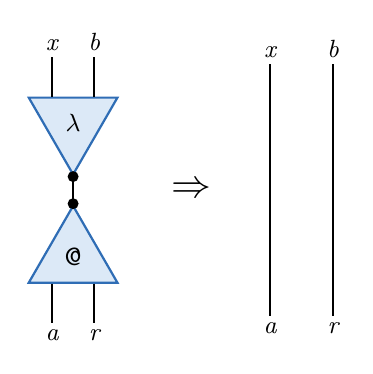
\begin{tikzpicture}
  \Down{l}{0,.85}{$\lambda$}{2}
  \Up{a}{0,-.85}{@}{2}
  \draw[wire] (l-0) -- (a-0);
  \draw[wire] (l-1) -- ++(0,.5) node[lbl,above] {x};
  \draw[wire] (l-2) -- ++(0,.5) node[lbl,above] {b};
  \draw[wire] (a-1) -- ++(0,-.5) node[lbl,below] {a};
  \draw[wire] (a-2) -- ++(0,-.5) node[lbl,below] {r};
  \ruleto{1.5,0}
  \draw[wire] (2.5,1.6) node[lbl,above] {x} -- (2.5,-1.6) node[lbl,below] {a};
  \draw[wire] (3.3,1.6) node[lbl,above] {b} -- (3.3,-1.6) node[lbl,below] {r};
\end{tikzpicture}
\hspace{1.8cm}
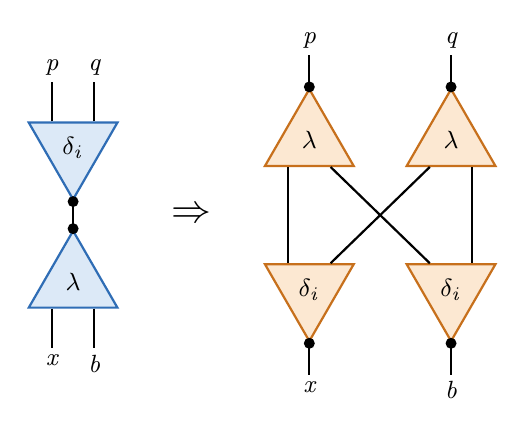
\begin{tikzpicture}
  \Down{d}{0,.85}{$\delta_i$}{2}
  \Up{l}{0,-.85}{$\lambda$}{2}
  \draw[wire] (d-0) -- (l-0);
  \draw[wire] (d-1) -- ++(0,.5) node[lbl,above] {p};
  \draw[wire] (d-2) -- ++(0,.5) node[lbl,above] {q};
  \draw[wire] (l-1) -- ++(0,-.5) node[lbl,below] {x};
  \draw[wire] (l-2) -- ++(0,-.5) node[lbl,below] {b};
  \ruleto{1.5,0}
  \Up[newagent]{l1}{3,.95}{$\lambda$}{2}
  \Up[newagent]{l2}{4.8,.95}{$\lambda$}{2}
  \Down[newagent]{d1}{3,-.95}{$\delta_i$}{2}
  \Down[newagent]{d2}{4.8,-.95}{$\delta_i$}{2}
  \draw[wire] (l1-0) -- ++(0,.4) node[lbl,above] {p};
  \draw[wire] (l2-0) -- ++(0,.4) node[lbl,above] {q};
  \draw[wire] (d1-0) -- ++(0,-.4) node[lbl,below] {x};
  \draw[wire] (d2-0) -- ++(0,-.4) node[lbl,below] {b};
  \draw[wire] (l1-1) -- (d1-1);
  \draw[wire] (l1-2) -- (d2-1);
  \draw[wire] (l2-1) -- (d1-2);
  \draw[wire] (l2-2) -- (d2-2);
\end{tikzpicture}
\caption{Left: $\beta$-reduction, $\Lam\act\App$. Right: a fan copies an
abstraction, $\Dup_i\act\Lam$. The variable and the body of the two copies
are joined by two new fans with the same label.}
\label{fig:beta}
\end{figure}

\noindent
The linear $\lambda$-calculus is not very expressive, since every function
uses its argument exactly once. But it is already enough to see why the
encoding works: a linear term \emph{is} a net, with $\Lam$ and $\App$ agents
for its constructs and wires for its variables, and its reductions are the
interactions of the net.

\subsection{Erasing}

A variable that does not occur, as in $\lambda x\,y.\,x$, leaves the
variable port of its $\Lam$ unconnected. The translation attaches an $\Era$
there. When an argument is passed to that $\lambda$, the $\Era$ meets it and
takes it apart:
\begin{lstlisting}
Era >< Lam(x, b)   => x ~ Era, b ~ Era
Era >< App(a, r)   => a ~ Era, r ~ Era
Era >< Era         =>
\end{lstlisting}
Note the rule for $\App$. An eraser that reaches the principal port of an
application (the function side) erases the application, sending erasers to
its argument and its result. Erasing in an interaction net is just as
incremental as everything else.

\subsection{Sharing: fans}

A variable used $k > 1$ times is connected to its occurrences through a tree
of $k-1$ \emph{fans}, $\Dup$ agents with their principal port towards the
$\lambda$. When a value arrives at the root of the tree, the fans copy it,
one agent at a time. A fan passes through an abstraction as in
\cref{fig:beta}, and through an application in the same way:
\begin{lstlisting}
Dup{i}(p, q) >< Lam(x, b)  => p ~ Lam(x1, b1), q ~ Lam(x2, b2),
                              x ~ Dup{i}(x1, x2), b ~ Dup{i}(b1, b2)
Dup{i}(p, q) >< App(a, r)  => p ~ App(a1, r1), q ~ App(a2, r2),
                              a ~ Dup{i}(a1, a2), r ~ Dup{i}(r1, r2)
\end{lstlisting}
(The $\{i\}$ is a label, explained below.) Look closely at the new fan on the
variable port $x$. It is ``upside down'': its principal port faces $x$, that
is, the \emph{occurrences} of the variable, and its two auxiliary ports go to
the variables of the two copies. When an argument later arrives at those
occurrences, this fan meets it and copies it. A fan going down into a body
copies it; a fan coming back up through a variable merges two copies of the
variable into one. The two are the same agent, used in opposite directions.

Here is $(\lambda x.\,x\,x)\,(\lambda y.\,y)$ again, now with named agents. The
self-application has a fan with label 1:
\begin{lstlisting}[style=trace]
$ python3 inet.py -t lam/selfapp.lam
   0  App(Lam(w1, w1), out) ~ Lam(Dup{1}(App(w2, w3), w2), w3)
   1  Lam(w1, w1) ~ Dup{1}(App(w2, out), w2)
   2  Dup{1}(w1, w2) ~ Dup{1}(w3, w4),  Lam(w3, w1) ~ App(Lam(w4, w2), out)
   3  App(Lam(w1, w1), out) ~ Lam(w2, w2)
   4  out ~ Lam(w1, w1)
\end{lstlisting}
In step 2 the fan has copied the $\Lam$ of the identity, and two new fans,
one on the copies' variables and one on their bodies, face each other on the
wire $y$ that joined them. They \emph{annihilate}: the first copy's variable
is connected to the first copy's body, and the second to the second. That is
exactly right. Each copy of the identity has become a separate identity.

\subsection{When two fans meet}\label{sec:fans}

Step 2 shows the central difficulty of the encoding. When two fans meet
principal to principal, there are two possibilities:
\begin{itemize}[itemsep=2pt]
\item they are the two ends of one copying operation, as in step 2: one fan
  went down into a term, another came back up through it, and now they meet
  again. Then they must \emph{annihilate}, pairing the first outputs with each
  other and the second with each other;
\item they belong to two \emph{different} copying operations, for instance one
  fan copies a term that itself contains a fan. Then they must
  \emph{commute}: each copies the other, as $\gamma$ and $\delta$ do.
\end{itemize}
The two agents look the same, so the rule cannot tell which case applies
unless the agents carry more information. The simplest scheme gives every
fan a \emph{label}, the same for all the fans of one copying operation, and
writes two rules, the first taking precedence:
\begin{lstlisting}
Dup{i}(p, q) >< Dup{i}(s, t)  => p ~ s, q ~ t
Dup{i}(p, q) >< Dup{j}(s, t)  => p ~ Dup{j}(a, b), q ~ Dup{j}(c, d),
                                 s ~ Dup{i}(a, c), t ~ Dup{i}(b, d)
\end{lstlisting}
\texttt{inet.py} gives each $\lambda$ that needs fans a fresh label, and
labels are copied with the fans. This works for many terms. Applying the
Church numeral $2 = \lambda f\,x.\,f\,(f\,x)$ to itself gives $4$, correctly
(\texttt{lam/twotwo.lam}):
\begin{lstlisting}[style=trace]
$ python3 inet.py -c lam/twotwo.lam
\x y. x (x (x (x y)))
interactions: 14 (Dup-App 2, Dup-Dup 4, Dup-Lam 3, Lam-App 5)
normal order: 6 beta steps
check: ok
\end{lstlisting}
The option \texttt{-c} reduces the same term in normal order, with
substitution, and compares the results. But now share the numeral before
applying it to itself, $(\lambda n.\,n\,n)\,2$, which ought to give the same
answer (\texttt{lam/shared.lam}):
\begin{lstlisting}[style=trace]
$ python3 inet.py -c lam/shared.lam
\x y. ...
interactions: 16 (Dup-App 2, Dup-Dup 5, Dup-Lam 4, Lam-App 5)
normal order: 7 beta steps
check: WRONG
\end{lstlisting}
The trace shows what happened. After 9 interactions the net is
\begin{lstlisting}[style=trace]
   9  App(Lam(Dup{2}(App(w1, w2), App(w3, w1)), Lam(w3, w2)), out)
        ~ Lam(Dup{2}(App(w4, w5), App(w6, w4)), Lam(w6, w5))
\end{lstlisting}
which is $2\,2$, two copies of the numeral applied to each other. It is the
same net that \texttt{twotwo.lam} starts from, with one difference: there the
two numerals' fans have labels 2 and 1, and here both have label 2, because
both are copies of the same numeral. When the first numeral's fan begins to
copy the second numeral, it meets that numeral's fan, sees the same label,
and annihilates instead of commuting. The rest of the reduction goes wrong,
and ends in a vicious circle, $\Dup_2(w_3,w_4) \eqn w_4$.

The term $\Omega = (\lambda x.\,x\,x)\,(\lambda x.\,x\,x)$ fails in the same
way. It should reduce for ever, but under this scheme it stops after 11
interactions, in a net that is a vicious circle.

\subsection{The oracle, and optimal reduction}\label{sec:oracle}

Fresh labels per binder are not enough, because one fan may have to copy
another fan with the same origin. The correct information is not ``which
binder'' but ``at what \emph{depth} of copying'': how many enclosing copy
operations the fan is inside. Lamping's algorithm~\cite{lamping90} gives every
fan a \emph{level}, and adds \emph{bracket} and \emph{croissant} agents that
sit on the wires where a term enters or leaves the scope of a copy, and raise
or lower the levels of whatever passes through them. Two fans annihilate when
their levels are equal and commute otherwise, and the brackets keep the
levels consistent. These extra agents are called the \emph{oracle}, and their
interactions are pure bookkeeping, with no $\beta$-step among them.
Gonthier, Abadi and Lévy~\cite{gal92} explained the oracle through Girard's
geometry of interaction, and Asperti and Guerrini's book~\cite{ag98} is the
standard account. Lambdascope~\cite{lambdascope} is a later, simpler
formulation with a single kind of scope delimiter.

Without the oracle, using fans and levels alone, the algorithm is called
\emph{abstract}. It is correct for terms that can be typed in
\emph{elementary affine logic}, a logic with a restricted copying modality
whose box depths give the levels directly~\cite{coppolamartini06,bcd11}.
HVM~\cite{hvm} takes the practical route of \texttt{inet.py}: fans carry
labels chosen when the program is written, and programs whose fans would meet
themselves are simply not supported.

\paragraph{Why go to this trouble?} Because a correct fan discipline gives
\emph{optimal} reduction. Lévy~\cite{levy80} asked what the least amount of
work is to reach a normal form. Normal order may copy an unevaluated argument
and then reduce each copy separately; call-by-need shares arguments, but
still repeats work inside a $\lambda$ that is applied several times, such as
a redex inside the body that does not depend on the bound variable (full
laziness fixes some of these cases but not all). Lévy defined \emph{families}
of redexes, the redexes that are copies of one another in a precise sense,
and showed that a reduction that does each family in one step is optimal.
No term-based machine can do it, because the copies of a family's redexes
may be in different places of the term. A net does it naturally, because a
fan copies a term \emph{lazily}, one agent at a time: two copies share
everything that has not yet been pulled apart, including redexes, and a
$\beta$-interaction on the shared part counts for both copies at once.

\subsection{Reading the result back}

The normal form of a net is a net, and in general it still contains fans:
the normal form of $2\,2$ shares the variable $f$ of $\lambda f\,x.\,f\,(f\,(f\,(f\,x)))$
through a tree of three fans. To print it as a term, the readback walks from
the interface downwards, through $\Lam$ bodies and through both the function
and argument of each $\App$. It keeps, for each label, a stack of choices. On
entering a fan at auxiliary port $k$, coming up from one copy, it pushes $k$
and continues through the principal port; on entering a fan at its principal
port, going down into a shared part, it pops the top choice and leaves by that
auxiliary port. This retraces the path that the copy would have taken, and
reconstructs one occurrence at a time. A missing choice or a cycle means that
the net is not the image of a term, which is how \texttt{inet.py} reports
the failures of \cref{sec:fans}: it prints \texttt{...} for a cycle and a
name beginning with \texttt{?} for a missing choice.

\subsection{Measurements}\label{sec:measure}

\Cref{tab:measure} compares the net with normal-order reduction on terms for
which the fresh-label scheme is correct. The terms use the Church numerals,
booleans and pairs defined in the file \texttt{lam/church.lam}, with
$\mathit{pred}$ defined by the usual pairing trick, and
$\mathit{id} = \lambda x.\,x$. The column ``complete'' reduces the whole
net, in any order; ``lazy'' (option \texttt{-l}) reduces only the active
pairs that the readback reaches, as in \cref{sec:garbage}.

\begin{table}[t]
\centering
\begin{tabular}{@{}l r r r r r@{}}
\toprule
& normal order & \multicolumn{2}{c}{complete} & \multicolumn{2}{c}{lazy}\\
\cmidrule(lr){3-4}\cmidrule(l){5-6}
term & $\beta$ & $\beta$ & all & $\beta$ & all\\
\midrule
$\mathit{succ}\ 2$ & 3 & 3 & 3 & 3 & 3\\
$2\ 2$ & 6 & 5 & 14 & 5 & 14\\
$2\ 2\ 2\ \mathit{id}$ & 59 & 15 & 49 & 15 & 49\\
$3\ 2\ 2\ \mathit{id}$ & 973 & 20 & 84 & 20 & 84\\
$\mathit{iszero}\ (\mathit{times}\ 3\ 3)$ & 9 & 13 & 57 & 9 & 17\\
$\mathit{pred}\ 3$ & 36 & 41 & 186 & 30 & 105\\
$\mathit{iszero}\ (\mathit{pred}\ (\mathit{pred}\ 3))$ & 50 & 77 & 372 & 43 & 146\\
\bottomrule
\end{tabular}
\caption{$\beta$-steps of normal-order reduction against $\Lam\act\App$
interactions and all interactions of the net. ``Complete'' counts do not
depend on the order of reduction.}
\label{tab:measure}
\end{table}

\noindent
Three things stand out.

\begin{description}[itemsep=3pt, font=\normalfont\itshape]
\item[Sharing pays, sometimes enormously.] $3\,2\,2\,\mathit{id}$ computes
  $2^{2^3}$ applications of the identity, $256$, and normal order does each
  of them. The net shares them: 20 $\beta$-interactions instead of 973.
  Exponentials of Church numerals are the textbook case for optimal
  reduction, because the work is a tower of repeated applications of the
  same function.
\item[Bookkeeping is not free.] Most interactions are not $\beta$-steps but
  fan interactions: 64 of the 84 for $3\,2\,2\,\mathit{id}$. With the full
  oracle there would also be bracket interactions, often many more. Asperti
  and Mairson~\cite{am98} proved that the bookkeeping for one family can
  cost more than any elementary function (any fixed tower of exponentials)
  of the size of the term. Optimal means \emph{fewest} $\beta$-steps, not
  fastest.
\item[Garbage costs, unless the strategy avoids it.] For
  $\mathit{iszero}\ (\mathit{pred}\ (\mathit{pred}\ 3))$, complete reduction
  does 77 $\beta$-steps, more than normal order's 50, because it also
  reduces the parts of the pairs that $\mathit{fst}$ throws away. The lazy
  strategy skips them and does 43, fewer than normal order, with less than
  half of the total work.
\end{description}

% =====================================================================
\section{Implementing interaction nets}\label{sec:implementation}

\subsection{Representation}

An agent is a tag and $n+1$ port fields, where a port field names the
\emph{peer} port: the agent at the other end of the wire, and which of its
ports it is. Packing the port number into the low bits of the address is
natural: agents of arity up to 3 have at most 4 ports, which fits in the two
low bits of an address aligned to four words. A wire is not an object; it is
just the two port fields that point at each other. Free wires are ports of
special interface agents that never interact.

All agents can have the same size if the arity is bounded (2 is enough for
the $\lambda$-calculus and for the interaction combinators). Then memory can
be managed with a free list: a rule frees the two agents of its active pair
and allocates the agents of its right-hand side, usually reusing the two it
just freed. There is no garbage collector, because there is no garbage that
is not explicitly erased.

\subsection{The reduction loop}

The machine keeps a stack of active pairs. The basic operation is
\emph{link}: connect two ports, by making each point at the other, and if
both are principal ports, push the pair. Then
\begin{lstlisting}[style=plain]
while the stack is not empty:
    pop a pair (a, b)
    look up the rule for (tag a, tag b)
    allocate the agents of its right-hand side
    link their ports to each other and to the peers of a's and b's ports
    free a and b
\end{lstlisting}
Each rule is straight-line code: a fixed number of allocations and links. For
a fixed set of rules they can be compiled; \texttt{inet.py} instead
interprets the rules from their equations. To instantiate a right-hand side it
builds the new agents, then resolves each name to the two ports it connects.
A name from the left-hand side stands for the peer of an auxiliary port of the
old pair; when that peer is itself an auxiliary port of the other agent of
the pair, the two names are simply joined.

A lazy strategy needs a different loop: instead of a stack of all active
pairs, it walks from the interface along principal ports, as the readback
does, and rewrites the first pair it finds. \texttt{inet.py} restarts the
walk from the interface after each interaction, which makes it quadratic but
simple; a real implementation keeps the path on a stack, much as a graph
reducer keeps its spine.

\subsection{Existing systems}

Pinto~\cite{pinto00} designed sequential and concurrent abstract machines for
interaction nets, and Mackie~\cite{mackie04} showed that carefully designed
$\lambda$-evaluators built as interaction nets can be efficient in
practice. HVM~\cite{hvm} is a recent runtime, with the language Bend
on top, that compiles a functional language to a variant of the interaction
combinators with labelled fans, native numbers and a few extra agents, and
runs it in parallel on multi-core CPUs and GPUs.

\subsection{On VM16}

An interaction-net reducer would be a natural fourth machine for VM16, next
to the SECD machine, the CAM and the graph reducer. It has not been written,
but its outline is clear. An agent of arity 2 is four 16-bit words, a tag and
three ports; aligning agents to 8 bytes leaves the three low bits of a port
reference free for the port number. The active-pair stack can live on the
data stack. Memory needs only a free list. Native numbers and arithmetic
would be extra agents, as in HVM: a number agent of arity 0 carrying its
value, and an operator agent that waits for two numbers. The \texttt{.lam}
programs of the companion tutorials could then be measured in interactions
next to their SECD transitions, CAM instructions and graph reductions.

% =====================================================================
\section{Comparison}\label{sec:comparison}

\begin{center}
\small
\begin{tabularx}{\textwidth}{@{}l X X X@{}}
\toprule
& SECD and CAM & graph reduction & interaction nets\\
\midrule
sharing & environments, closures & pointers into a graph & explicit fans\\
copying & closures share code and environment & none; nodes are shared & incremental, one agent per step\\
garbage & collector & collector & explicit erasers\\
evaluation order & fixed (strict) & fixed (lazy, spine first) & irrelevant to the result and the number of steps\\
step cost & bounded per instruction & bounded per rule & bounded per rule\\
sharing under $\lambda$ & none & partial (full laziness) & optimal, with the oracle\\
parallelism & none & needs locking & natural\\
\bottomrule
\end{tabularx}
\end{center}

\noindent
The deepest difference is the last-but-one row. The SECD machine and the CAM
cannot share work inside a function body at all: each call evaluates the body
afresh. Graph reduction shares a whole argument, and with full laziness the
parts of a body that do not depend on the argument. Interaction nets with a
correct fan discipline share every family of redexes, which is the best that
is possible. The price is the bookkeeping of \cref{sec:measure}, which is why
practical systems either restrict the language, as HVM does, or use
interaction nets to implement a conventional strategy, as Mackie's
evaluators do.

% =====================================================================
\section{Summary}

\begin{itemize}[itemsep=2pt]
\item An interaction net is a graph of agents, each with one principal port,
  connected by wires. A rule rewrites two agents joined at their principal
  ports, and preserves the interface exactly.
\item Programs are written by giving one rule per pair of agents. A function
  inspects one argument, at its principal port; copying and erasing are
  agents with rules like any other.
\item Active pairs never overlap, so reduction is strongly confluent: every
  order gives the same result in the same number of steps, and all pairs can
  be reduced in parallel. The price is that complete reduction also reduces
  garbage, which a lazy strategy avoids.
\item Three agents, $\gamma$, $\delta$ and $\varepsilon$, can simulate every
  interaction system.
\item The $\lambda$-calculus is $\Lam$, $\App$, fans and erasers, with
  $\beta$ a single interaction. Deciding when two fans annihilate needs
  labels, and in general Lamping's oracle; with it, reduction is optimal in
  Lévy's sense, though the bookkeeping may dominate the cost.
\end{itemize}

% =====================================================================
\section*{Exercises}
\addcontentsline{toc}{section}{Exercises}

\begin{exercise}
Write rules for $\ag{Pred}$ (with $\mathit{pred}\ \Z = \Z$) and for
subtraction $\ag{Sub}$, which inspects its \emph{second} argument. How many
interactions does $m - n$ take?
\end{exercise}

\begin{exercise}
Write rules for an agent $\ag{Eq}$ that compares two numbers and produces
$\ag{True}$ or $\ag{False}$. You will need an intermediate agent, as for
$\ag{Max}$. What must happen to the unused parts of the numbers?
\end{exercise}

\begin{exercise}
Lists are $\ag{Nil}$ and $\ag{Cons}(h,t)$. Write rules for $\ag{Append}$,
and for $\ag{Dup}$ and $\ag{Era}$ on lists. Reduce
$\mathit{append}\ [1,2]\ [3]$ with \texttt{inet.py}.
\end{exercise}

\begin{exercise}\label{ex:dlist}
Represent a difference list by a pair of wires, its front and its end, and
write a net for the concatenation of two difference lists. How many
interactions does it take? Now write a rule that reverses an ordinary list
into a difference list, with an accumulator.
\end{exercise}

\begin{exercise}
Prove \cref{cor:length} from \cref{thm:confluence}. (Hint: induction on the
length of the shortest reduction to normal form.) Why does the corollary fail
for the $\lambda$-calculus?
\end{exercise}

\begin{exercise}
Find a net with an active pair whose reduction loops for ever without
growing, so that memory use stays bounded. Can a finite net in which no rule
has an active pair on its right-hand side reduce for ever?
\end{exercise}

\begin{exercise}
Check that $\gamma\act\gamma$ must cross its wires for
$\gamma(x,b)$ and $\gamma(r,a)$ to encode $\beta$-reduction, as in
\cref{sec:combinators}. What would go wrong with uncrossed wires?
\end{exercise}

\begin{exercise}
Draw the net for $(\lambda x.\,x\,x)\,(\lambda y.\,y)$ as a picture, then
reduce it by hand, and compare with the trace in \cref{sec:lambda}.
\end{exercise}

\begin{exercise}
Run \texttt{inet.py -t lam/shared.lam} and find the first interaction that
goes wrong. Which fans should have commuted?
\end{exercise}

\begin{exercise}
Using \texttt{inet.py -c}, find the smallest term you can for which the
fresh-label scheme gives a wrong answer. Is there one without
self-application?
\end{exercise}

\begin{exercise}
Add native numbers to \texttt{lambda.inet}: an agent $\ag{Num}_n$ for each
number, and agents for $+$ that wait for two numbers. How are numbers copied
and erased?
\end{exercise}

% =====================================================================
\section{Reference card}\label{sec:card}

\paragraph{Notation.} $\alpha(t_1,\dots,t_n)$: an agent whose principal port
is the root and whose auxiliary ports are connected to $t_1,\dots,t_n$. A
name: a wire (twice in a rule or net) or an interface wire (once in a net).
$t \eqn u$: connect two roots. $\alpha(\vec x)\act\beta(\vec y) \rul \Delta$:
a rule.

\paragraph{Unary numbers} (\texttt{nat.inet}).
\begin{lstlisting}
Add(r, y) >< Z      => r ~ y
Add(r, y) >< S(x)   => r ~ S(w), x ~ Add(w, y)
Mul(r, y) >< Z      => r ~ Z, y ~ Era
Mul(r, y) >< S(x)   => y ~ Dup(a, b), x ~ Mul(m, a), m ~ Add(r, b)
Dup(a, b) >< Z      => a ~ Z, b ~ Z
Dup(a, b) >< S(x)   => a ~ S(a1), b ~ S(b1), x ~ Dup(a1, b1)
Era >< Z            =>
Era >< S(x)         => x ~ Era
\end{lstlisting}

\paragraph{Interaction combinators} (\texttt{combinators.inet}).
\begin{lstlisting}
Con(a, b) >< Con(c, d)  => a ~ d, b ~ c
Dup(a, b) >< Dup(c, d)  => a ~ c, b ~ d
Con(a, b) >< Dup(c, d)  => a ~ Dup(p, q), b ~ Dup(r, s),
                           c ~ Con(p, r), d ~ Con(q, s)
Era >< Con(a, b)        => a ~ Era, b ~ Era
Era >< Dup(a, b)        => a ~ Era, b ~ Era
Era >< Era              =>
\end{lstlisting}

\paragraph{The \texorpdfstring{$\lambda$}{lambda}-calculus} (\texttt{lambda.inet}).
$\Lam(x,b)$: principal port the function. $\App(a,r)$: principal port the
function, $a$ the argument, $r$ the result.
\begin{lstlisting}
Lam(x, b) >< App(a, r)       => x ~ a, b ~ r
Dup{i}(p, q) >< Dup{i}(s, t) => p ~ s, q ~ t
Dup{i}(p, q) >< Dup{j}(s, t) => p ~ Dup{j}(a, b), q ~ Dup{j}(c, d),
                                s ~ Dup{i}(a, c), t ~ Dup{i}(b, d)
Dup{i}(p, q) >< Lam(x, b)    => p ~ Lam(x1, b1), q ~ Lam(x2, b2),
                                x ~ Dup{i}(x1, x2), b ~ Dup{i}(b1, b2)
Dup{i}(p, q) >< App(a, r)    => p ~ App(a1, r1), q ~ App(a2, r2),
                                a ~ Dup{i}(a1, a2), r ~ Dup{i}(r1, r2)
Era >< Lam(x, b)             => x ~ Era, b ~ Era
Era >< App(a, r)             => a ~ Era, r ~ Era
Era >< Dup{i}(p, q)          => p ~ Era, q ~ Era
Era >< Era                   =>
\end{lstlisting}

\paragraph{Commands.}
\begin{lstlisting}[style=plain]
python3 inet.py [-t] [-q] [-r SEED] [-n LIMIT] prog.inet
python3 inet.py [-t] [-c] [-l] prog.lam       # -c check, -l lazy
sh test.sh
\end{lstlisting}

% =====================================================================
\begin{thebibliography}{99}

\bibitem{ag98}
A.~Asperti and S.~Guerrini.
\newblock \emph{The Optimal Implementation of Functional Programming
  Languages}.
\newblock Cambridge University Press, 1998.

\bibitem{am98}
A.~Asperti and H.~G. Mairson.
\newblock Parallel beta reduction is not elementary recursive.
\newblock In \emph{POPL}, 1998.

\bibitem{bcd11}
P.~Baillot, P.~Coppola, and U.~Dal~Lago.
\newblock Light logics and optimal reduction: completeness and complexity.
\newblock \emph{Information and Computation}, 209(2), 2011.

\bibitem{coppolamartini06}
P.~Coppola and S.~Martini.
\newblock Optimizing optimal reduction: a type inference algorithm for
  elementary affine logic.
\newblock \emph{ACM Transactions on Computational Logic}, 7(2), 2006.

\bibitem{fm99}
M.~Fernández and I.~Mackie.
\newblock A calculus for interaction nets.
\newblock In \emph{Principles and Practice of Declarative Programming (PPDP)},
  volume 1702 of \emph{LNCS}, pages 170--187. Springer, 1999.

\bibitem{girard87}
J.-Y. Girard.
\newblock Linear logic.
\newblock \emph{Theoretical Computer Science}, 50(1):1--102, 1987.

\bibitem{gal92}
G.~Gonthier, M.~Abadi, and J.-J. Lévy.
\newblock The geometry of optimal lambda reduction.
\newblock In \emph{POPL}, pages 15--26, 1992.

\bibitem{hvm}
V.~Taelin.
\newblock HVM, the Higher-order Virtual Machine.
\newblock \url{https://github.com/HigherOrderCO/HVM}.

\bibitem{lafont90}
Y.~Lafont.
\newblock Interaction nets.
\newblock In \emph{POPL}, pages 95--108, 1990.

\bibitem{lafont97}
Y.~Lafont.
\newblock Interaction combinators.
\newblock \emph{Information and Computation}, 137(1):69--101, 1997.

\bibitem{lamping90}
J.~Lamping.
\newblock An algorithm for optimal lambda calculus reduction.
\newblock In \emph{POPL}, pages 16--30, 1990.

\bibitem{levy80}
J.-J. Lévy.
\newblock Optimal reductions in the lambda-calculus.
\newblock In J.~P. Seldin and J.~R. Hindley, editors, \emph{To H.~B. Curry:
  Essays on Combinatory Logic, Lambda Calculus and Formalism}, pages
  159--191. Academic Press, 1980.

\bibitem{mackie04}
I.~Mackie.
\newblock Efficient $\lambda$-evaluation with interaction nets.
\newblock In \emph{Rewriting Techniques and Applications (RTA)}, volume 3091
  of \emph{LNCS}, pages 155--169. Springer, 2004.

\bibitem{pinto00}
J.~S. Pinto.
\newblock Sequential and concurrent abstract machines for interaction nets.
\newblock In \emph{Foundations of Software Science and Computation Structures
  (FoSSaCS)}, volume 1784 of \emph{LNCS}. Springer, 2000.

\bibitem{lambdascope}
V.~van Oostrom, K.-J. van de Looij, and M.~Zwitserlood.
\newblock Lambdascope: another optimal implementation of the
  lambda-calculus.
\newblock In \emph{Workshop on Algebra and Logic on Programming Systems
  (ALPS)}, 2004.

\end{thebibliography}

\end{document}
